\section*{Численные эксперименты}
\addcontentsline{toc}{subsection}{Численные эксперименты}

Тестирование проводилось на компьютере со следующими характеристиками:

\begin{center}
\begin{tabular}{| c | c |}
    \hline
    Частота процессора & 3.7 ГГц \\ \hline
    Архитектура & 64-битная \\ \hline
    Модель процессора & Intel(R) Xeon(R) CPU E5-1620 v2 \\ \hline
    Число ядер & 8 \\ \hline
    Оперативная память & 64 Гб \\ \hline
    Объём жёсткого диска & 300 Гб \\
    \hline
\end{tabular}
\end{center}
\bigskip

Старой реализацией будем называть
изначальную реализацию,
где для вычисления функционала
на векторе параметров запускался
новый интерпретатор и
заново происходила загрузка
функции скрипта.

Новым вариантом реализации
будем называть реализацию,
где используется очередь задач
и пул потоков,
интерпретаторы инициализируются
один раз и не подвергаются перезапуску,
то есть время жизни интерпретатора
завершается с окончанием
вычислений функционала.

План тестирования заключался
в сравнение времени работы
старой и новой реализаций
при одинаковых параметрах.
Проводились многократные запуски
с целью подтверждения или опровержения
гипотезы о статистической значимости различий
времени работы реализаций.
Под нулевой гипотезой будет пониматься
различие математического ожидания
старой и новой реализаций.

Первым этапом численного эксперимента
было получение замеров времени
работы приложения
при различных комбинациях параметров.

Параметрами были выбраны следующие характеристики:

\begin{itemize}
    \item \textbf{Число потоков (\textit{i})}

        Для новой реализации этот параметр также
        обозначал размер пула потоков.
        Диапазон значений: 1-8.
    \item \textbf{Коэффициент размера популяции (\textit{M})}

        Размер популяции рационально выбирать
        пропорционально числу потоков,
        чтобы на каждый поток приходилась
        равная нагрузка при различном
        числе \textit{i}.

        Таким образом размер популяции равен:
        \begin{math}M * i\end{math}

        Тестирование проходило для значений:
        \begin{math}M = 5; M = 10\end{math}.
\end{itemize}

\break
На следующих графиках представлены результаты тестирования:

\noindent
\begin{center}
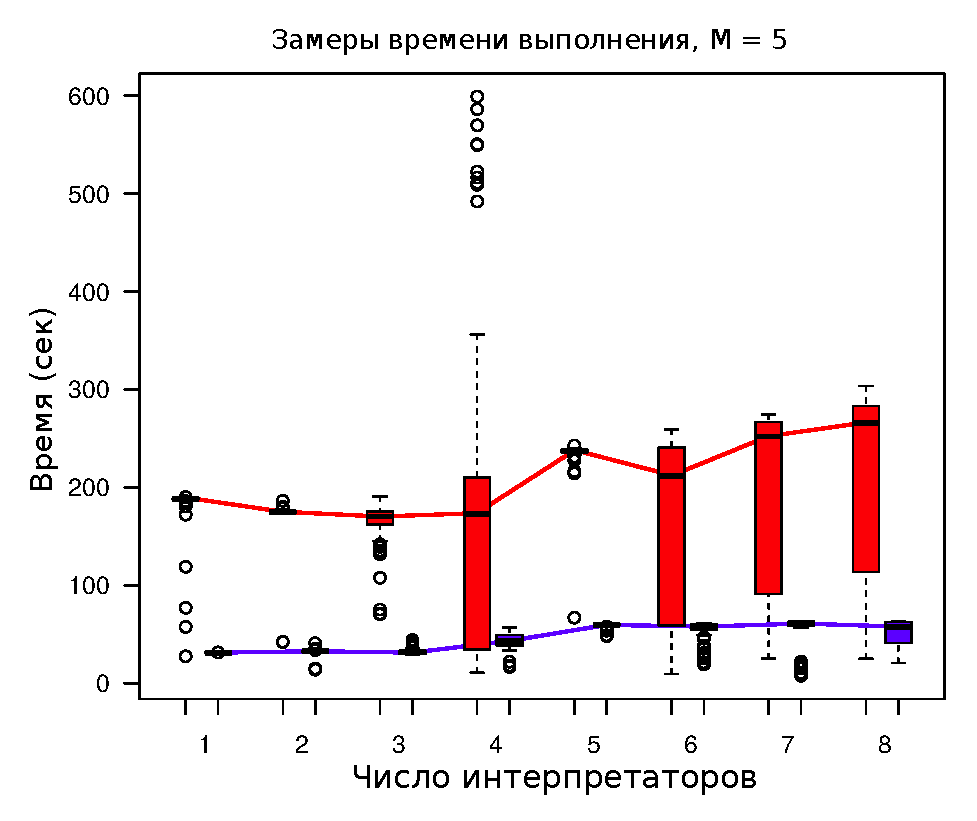
\includegraphics[width=0.85\textwidth]{m5}
\end{center}

\noindent
\begin{center}
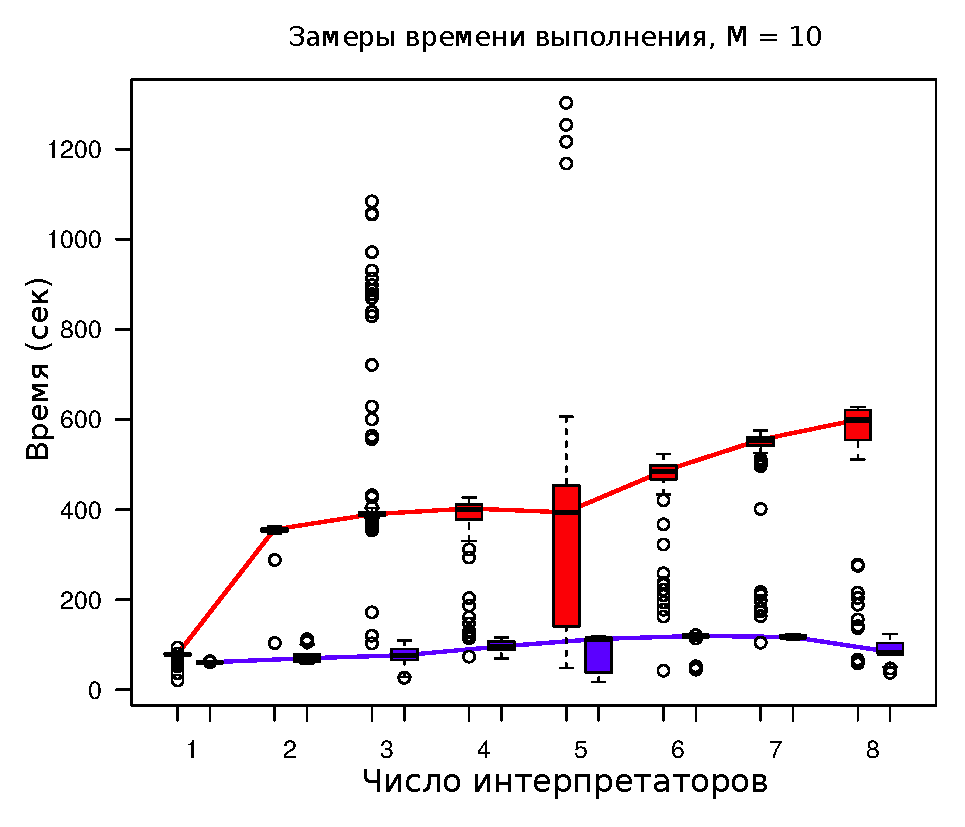
\includegraphics[width=0.85\textwidth]{m10}
\end{center}

Было проверено, оказывает ли изучаемый параметр,
в данном случае это новый вариант реализации,
существенное влияние на интересующую нас
переменную, на время работы.
Проверка осуществлялась с помощью
критерия достоверно значимой
разности Тьюки
с уровнем значимости в 95\%.
Он необходим, чтобы посмотреть
где именно лежат статистические различия.

\bigskip
\begin{center}
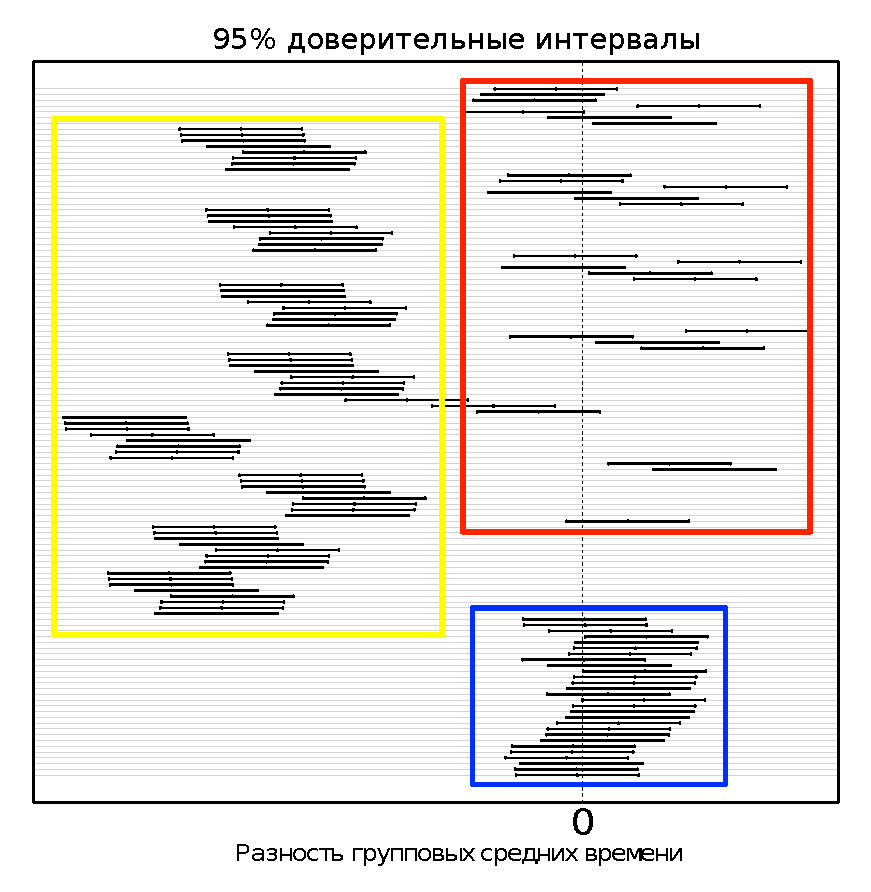
\includegraphics{tukey}
\end{center}

Пунктирной вертикальной линией показана
нулевая разница между групповыми средними времени.
Если доверительный интервал включает 0,
это указывает на отсутствие различий
между соответствующими группами.

На графике выделены три группы цветными рамками:
\begin{itemize}
    \item \textbf{Интервалы внутри красной рамки (справа вверху)} ---
        пары групп старой реализации с различным числом интерпретаторов.
        Интервалы лежат возле нуля, но присутствует
        некоторое разница, как в положительную сторону,
        так и в отрицательную. Это может объясняться
        конкуренцией интерпретаторов
        за вычислительные ресурсы и доступ к конфигурационным файлам
        при их одновременной инициализации.
    \item \textbf{Интервалы внутри синей рамки (справа внизу)} ---
        пары групп новой реализации с различным числом интерпретаторов.
        В данной группе различия минимальны,
        что является свидетельством оптимизации.
        В новой реализации инициализация интерпретаторов
        происходит единожды, поэтому
        узкое место не сильно замедляет работу
        при конкуренции, в дальнейшем
        интерпретаторы не так конкурируют за ресурсы.
    \item \textbf{Интервалы внутри жёлтой рамки (слева)} ---
        смешанные группы новой и старой реализации.
        Разница статистически значима,
        это означает, что оптимизация играет существенную роль.
\end{itemize}

